\documentclass[../main.tex]{subfiles}

%TODO

\begin{document}

\chapter{Розробка і тестування системи}

\section{Розробка системи}

На сьогоднішній момент об'єктно-\linebreak[0]орієнтований підхід є одним із напрямків в проектуванні систем, що швидко розвивається. Прикладом можуть бути об'єктно-\linebreak[0]орієнтований аналіз — методологія розробки систем, запропонована Йорденом, об'єктно-орієнтоване проектування, об'єктно-\linebreak[0]орієнтоване програмування, реалізоване в численних компіляторах C++, Object Pascal, Borland Pascal, Smalltalk.

Основу ООП складають три основні концепції: інкапсуляція, успадкування та поліморфізм. Одною з переваг ООП є краща модульність програмного забезпечення (тисячу функцій процедурної мови, в ООП можна замінити кількома десятками класів із своїми методами). Сьогодні багато мов програмування або підтримують ООП (PHP, Lua) або ж є цілком об'єктно-орієнтованими (зокрема, Java, C\#, C++, Python, Ruby та Objective-C, ActionScript 3, Swift, Vala).

На відміну від традиційних поглядів, коли програму розглядали як набір підпрограм, або як перелік інструкцій комп'ютеру, ООП програми можна вважати сукупністю об'єктів. Відповідно до парадигми об'єктно-\linebreak[0]орієнтованого програмування, кожний об'єкт здатний отримувати повідомлення, обробляти дані, та надсилати повідомлення іншим об'єктам. Кожен об'єкт — своєрідний незалежний автомат з окремим призначенням та відповідальністю \cite{object_oriented_analysis}.

ООП виникло в результаті розвитку ідеології процедурного програмування, де дані і підпрограми (процедури, функції) їх обробки формально не пов'язані. Для подальшого розвитку об'єктно-орієнтованого програмування велике значення мають поняття події (так зване подієво-орієнтоване програмування) і компоненти (компонентне програмування,~КОП).

Формування КОП від ООП відбулося, так само як формування модульного від процедурного програмування: процедури сформувалися в модулі — незалежні частини коду до рівня збірки програми, так об'єкти сформувалися в компоненти — незалежні частини коду до рівня виконання програми. Взаємодія об'єктів відбувається за допомогою повідомлень. Результатом подальшого розвитку ООП, мабуть, буде агентно-орієнтоване програмування, де агенти — незалежні частини коду на рівні виконання. Взаємодія агентів відбувається за допомогою зміни середовища, в якій вони знаходяться.

Мовні конструкції, конструктивно не пов'язані безпосередньо з об'єктами, але необхідні їм для їх безпечної (виняткові ситуації, перевірки) та ефективної роботи, інкапсулюються від них в аспекти (в~аспектно-\linebreak[0]орієнтованому програмуванні). Суб'єктно-орієнтоване програмування розширює поняття об'єктів шляхом забезпечення більш уніфікованого і незалежної взаємодії об'єктів. Може бути перехідною стадією між ООП та агентним програмуванням в частині самостійної їх взаємодії.

\subsection{Обґрунтування вибору засобів реалізації}

Для реалізації серверної частини програмного комплексу багтрекінгової системи було використано:
\begin{enumerate}
	\item Swagger -- формалізована специфікація і екосистема безлічі інструментів, що надає інтерфейс між front-end системами, кодом бібліотек низького рівня і комерційними рішеннями у вигляді API. Разом з тим, специфікація побудована таким чином, що не залежить від мов програмування, і зручна у використанні як людиною, так і машиною \cite{swagger}.
	\item REST -- підхід до архітектури мережевих протоколів, які забезпечують доступ до інформаційних ресурсів.
	\item JSON -- текстовий формат обміну даними між комп'ютерами. Базується на тексті, може бути прочитаним людиною. Формат дозволяє описувати об'єкти та інші структури даних.
	\item Node.js -- платформа з відкритим кодом для виконання високопродуктивних мережевих застосунків, написаних мовою JavaScript.
	\item JavaScript -- динамічна, об'єктно-орієнтована мова програмування. Реалізація стандарту ECMAScript.
	\item MariaDB -- реляційна система керування базами даних, створена на початку 2009 як відгалуження (форк) MySQL.
\end{enumerate}

Вибір Swagger'у в ролі фреймворку специфікації обумовлений тим, що на даний момент це єдиний абсолютно безкоштовний та підтримуваний фреймворк даного типу. Його використання дозволило значно пошвидшити розробку системи, надаючи методи з генерації робочих моделей даних та каркасів роботи з ними для конкретних платформ розробки. Щодо призначення, OpenAPI розглядається як універсальний інтерфейс для користувачів (клієнтів) по взаємодії з сервісами (серверами). Якщо спроектована специфікація для деякого сервісу, то на її підставі можна генерувати вихідний код для бібліотек клієнтських додатків, текстову документацію для користувачів, варіанти тестування та ін. Для цих дій є великий набір інструментів для різних мов програмування і платформ.

Swagger специфікація не залежить від мови програмування, і може бути використана поза протоколом HTTP. OpenAPI одночасно застосовується для клієнта, сервера і відповідної документації інтерфейсу, створеного відповідно до REST. Специфікація декларативна, і тому може бути використана клієнтами без знань особливостей серверної реалізації. При цьому працювати з OpenAPI можуть як розробники, так і рядові користувачі через готові інструменти % TODO как-то оно не является одним предложением
і надаються інтерфейси. Як формат використовується XML і JSON, але в загальному випадку може бути обрана й інша мова розмітки.

В якості стилю обміну даними між клієнотом та сервером було вибрано REST з таких причин:
\begin{enumerate}
	\item Легкість.
	\item Простота в обслуговуванні.
	\item Масштабованість і гнучкість.
	\item Ефективність і швидкість.
	\item Висока продуктивність.
	\item Споживання низької кількості трафіку.
	\item Можливість використання без дорогих сторонніх інструментів.
\end{enumerate}
Окрім цього, в основі REST закладено принципи функціонування Всесвітньої павутини і, зокрема, можливості HTTP. Філдінг розробив REST паралельно з HTTP 1.1 базуючись на попередньому протоколі HTTP 1.0.

REST, як і кожен архітектурний стиль відповідає ряду архітектурних обмежень. Це гібридний стиль який успадковує обмеження з інших архітектурних стилів.

Перша архітектура від якої він успадковує обмеження — це клієнт-серверна архітектура. Її обмеження вимагає розділення відповідальності між компонентами які займаються зберіганням та оновленням даних (сервером) і тими компонентами які займаються відображенням даних на інтерфейсі користувача та реагування на дії з цим інтерфейсом (клієнтом). Таке розділення дозволяє компонентам еволюціонувати незалежно.

Наступним обмеженням є те, що взаємодії між сервером та клієнтом не~мають стану, тобто кожен запит містить всю необхідну інформацію для його обробки, і не~покладається на те, що сервер знає щось з попереднього запиту. Таким чином, наприклад дані про стан сесії (користувача який аутентифікувався) зберігаються на клієнті, і передаються з кожним запитом. Це покращує масштабовність, бо сервер після закінчення обробки запиту може звільнити всі ресурси задіяні для цієї операції, без жодного ризику втратити цінну інформацію. Також спрощується моніторинг і зневадження, бо для того, аби розібратись, що відбувається в певному запиті, досить подивитись лише на той один запит. Збільшується надійність, бо помилка в одному запиті не~зачіпає інші.

Мінусом цього обмеження є те, що знижується продуктивність, через те що в кожен запит тепер доводиться додавати дані сесії з клієнта. Також збереження стану на різних клієнтах важче підтримувати, бо реалізації клієнтів можуть відрізнятись, в той час як середовище сервера повністю під контролем розробника.

Додатковим обмеженням стилю REST є те, що системи написані в цьому стилі повинні підтримувати кешування, тобто дані які передаються між сервером % TODO між сервером і ким?
повинні містити інформацію про те, чи можна їх кешувати, і якщо можна, то як довго. Це дозволяє збільшувати продуктивність, уникаючи зайвих запитів, але також зменшує надійність системи, через те, що дані в кеші можуть бути застарілі.

Рання архітектура веб, створена Тімом Бернерсом-Лі, відповідала цим трьом обмеженням — клієнт-сервер без стану з підтримкою кешування. Проте стиль REST додає ще додаткові обмеження.

Всі компоненти в архітектурі REST підтримують однорідний інтерфейс. Це зменшує зв'язність між компонентами і сервісами які вони надають і дозволяє нескладно змінювати компоненти при потребі.[5] Це досягається кількома точнішими обмеженнями:

\begin{itemize}
	\item ідентифікація ресурсів;
	\item маніпуляція ресурсами через представлення;
	\item самоописові повідомлення;
	\item гіпермедіа як рушій стану застосунку.
\end{itemize}

Наступним обмеженням для REST є поділ на шари абстракції. Кожен компонент потрапляє в якийсь шар, і спілкується лише з компонентами в шарі під ним або в шарі над ним. Обмежнення знання системи одним шаром зменшує складність компонентів.

Останнім архітектурним обмеженням в REST є те, що клієнти повинні дозволяти розширювати свою функціональність, дозволяючи завантаження додаткового коду (code on demand[en]) у~формі аплетів чи скриптів. Це~спрощує клієнти, дозволяючи не~реалізовувати всі необхідні функції попередньо. Щоправда це необов'язкове обмеження, і якщо воно не дає переваг для конкретного застосування, то його не обов'язково реалізовувати. Наприклад, дозвіл завантаження стороннього коду може бути не бажаним з точки зору безпеки.

Компоненти REST системи спілкуються, передаючи один одному представлення ресурсу в форматі, що обирається з оновлюваного набору стандартних форматів даних. Формат обирається динамічно відповідно до бажань компонента-клієнта і можливостей сервера. Чи представлення має той самий формат, що й сам ресурс, чи є результатом якогось перетворення\nolinebreak[2] — це деталь реалізації, яка ховається за інтерфейсом.

Ресурс — це ключовий елемент даних в REST. Ресурсом може бути що завгодно, що можна назвати: якийсь документ (наприклад додаток до звіту), динамічне значення (наприклад інформація щодо проекту), щось з реального світу (наприклад інформація щодо учасника проекту).

Для того, щоб посилатись на ресурси, використовуються ідентифікатори ресурсів. Компонент, який надав ресурсу ідентифікатор і дозволяє звертатись до нього за цим ідентифікатором, відповідає за збереження функції приналежності незмінною. Якість ідентифікатора залежить від якості компонента, який цей ідентифікатор надає, тому деякі ідентифікатори стають «мертвими посиланнями», коли інформацію переміщують або знищують.

В якості формату обміну даними між клієнтом та сервером було вибрано JSON з таких причин:
\begin{enumerate}
	\item Малий розмір повідомлення.
	\item Гарно структурована інформація в документі.
	\item Легко розрізняти типи даних.
	\item Можна легко розрізняти окремі предмети і колекції розміром в один елемент.
	\item Легко передати null-значення.
	\item Легко споживається % TODO maybe обробляти 
	за допомогою JavaScript.
\end{enumerate}

За рахунок своєї лаконічності в порівнянні з XML, формат JSON може бути більш придатним для серіалізації складних структур.

JSON будується на двох структурах:
\begin{enumerate}
	\item Набір пар ім'я/значення. У різних мовах це реалізовано як об'єкт, запис, структура, словник, хеш-таблиця, список з ключем або асоціативним масивом. % TODO maybe або асоціативний масив
	\item Впорядкований список значень. У багатьох мовах це реалізовано як масив, вектор, список, або послідовність.
\end{enumerate}

Це універсальні структури даних. Теоретично всі сучасні мови програмування підтримують їх у тій чи іншій формі. Оскільки JSON використовується для обміну даними між різними мовами програмування, то є сенс будувати його на цих структурах.

У JSON використовуються такі їхні форми:
\begin{enumerate}
	\item Об'єкт — це послідовність пар ім'я/значення. Об'єкт починається з символу \{ і закінчується символом \}. Кожне значення слідує за : і пари ім'я/значення відділяються комами.
	\item Масив — це послідовність значень. Масив починається символом [ і закінчується символом ]. Значення відділяються комами.
	\item Значення може бути рядком в подвійних лапках, або числом, або логічними true чи false, або null, або об'єктом, або масивом. Ці\nolinebreak[3] структури можуть бути вкладені одна в одну.
	\item Рядок — це послідовність з нуля або більше символів юнікода, обмежена подвійними лапками, з використанням escape-\linebreak[0]послідовностей, що починаються із зворотної косої риски (backslash). Символи представляються простим рядком.
\end{enumerate}

Тип Рядок (String) дуже схожий на String в мовах C і Java. Число теж дуже схоже на C- або Java-число, за винятком того, що вісімкові та шістнадцяткові формати не використовуються. Пропуски можуть бути вставлені між будь-якими двома лексемами.

Node.js було вибрано у ролі середовища виконання серверного додатку тому, що це найбільш популярна, стабільна та ефективна реалізація серверного середовища виконання JavaScript коду.\pagebreak[2] % фактически чтоб уменьшить риск отрыва следующего абзаца (являющегося по сути заголовком списка) от самогО списка. Увы, поставить там \nopagebreak не~работает

Node.js характеризується такими властивостями:
\begin{enumerate}
	\item Асинхронна однопотокова модель виконання запитів.
	\item Неблокуючий ввід/вивід.
	\item Система модулів CommonJS.
	\item Рушій JavaScript Google V8.
\end{enumerate}

Node.js призначений для відокремленого виконання високопродуктивних мережних застосунків на мові JavaScript. Функції платформи не обмежені створенням серверних скриптів для веб, платформа може використовуватися і для створення звичайних клієнтських і серверних мережевих програм. Для забезпечення виконання JavaScript-коду використовується розроблений компанією Google рушій V8.

Для забезпечення обробки великої кількості паралельних запитів у Node.js використовується асинхронна модель запуску коду, заснована на обробці подій в неблокуючому режимі та визначенні обробників зворотніх викликів (callback). Як способи мультиплексування з'єднань підтримується epoll, kqueue, /dev/poll і select. Для мультиплексування з'єднань використовується бібліотека libuv, для створення пулу потоків (thread pool) задіяна бібліотека libeio, для виконання DNS-запитів у неблокуючому режимі інтегрований c-ares. Всі системні виклики, що спричиняють блокування, виконуються всередині пула потоків і потім, як і обробники сигналів, передають результат своєї роботи назад через неіменовані канали~(pipe). % to avoid too short last line

Для розширення функціональності застосунків на базі Node.js підготовлена велика колекція модулів, в якій можна знайти реалізацію HTTP, SMTP, XMPP, DNS, FTP, IMAP, POP3 серверів і клієнтів, модулі для інтеграції з різними веб-фреймворками, обробники WebSocket і AJAX, конектори до СУБД (MySQL, PostgreSQL, SQLite, MongoDB), шаблонізатори, CSS-рушії, реалізації криптоалгоритмів і систем авторизації (наприклад, OAuth), XML-парсери.

JavaScript було вибрано як мову реалізації серверної частини з таких причин:
\begin{enumerate}
	\item Можливість використовувати одну й ту саму мову програмування як на сервері, так і на клієнті.
	\item Висока швидкість у зв'язці з Node.js.
	\item Підтримка JSON об'єктів без необхідності в створенні будь-яких моделей для опису повідомлень.
	\item Можливість прямого зв'язування зі Swagger специфікацією без потреби в написанні додаткового коду.
	\item Динамічна типізація, що дозволяє розроблювати систему швидше та додає їй гнучкості.
\end{enumerate}

JavaScript класифікують як прототипну (підмножина об'єктно-\linebreak[0]орієнтованої) скриптову мову програмування з динамічною типізацією. Окрім прототипної, JavaScript також частково підтримує інші парадигми програмування (імперативну та частково функціональну) і деякі відповідні архітектурні властивості, зокрема: динамічна та слабка типізація, автоматичне керування пам'яттю, прототипне наслідування, функції як об'єкти першого класу.

Незважаючи на схожість назв, мови Java та JavaScript є двома різними мовами, що мають відмінну семантику, хоча й мають схожі риси в стандартних бібліотеках та правилах іменування. Синтаксис обох мов отриманний «у спадок» від мови С, але семантика та дизайн JavaScript є результатом впливу мов Self та Scheme.

JavaScript має низку властивостей об'єктно-орієнтованої мови, але завдяки концепції прототипів підтримка об'єктів в ній відрізняється від традиційних мов ООП. Крім того, JavaScript має ряд властивостей, притаманних функціональним мовам — функції як об'єкти першого класу, об'єкти як списки, каррінг, анонімні функції, замикання (closures) — що додає мові додаткову гнучкість.

JavaScript має C-подібний синтаксис, але в порівнянні з мовою С має такі корінні відмінності:
\begin{enumerate}
	\item Об'єкти, з можливістю інтроспекції і динамічної зміни типу через механізм прототипів.
	\item Функції як об'єкти першого класу.
	\item Обробка винятків.
	\item Автоматичне приведення типів.
	\item Автоматичне прибирання сміття.
	\item Анонімні функції.
\end{enumerate}

JavaScript містить декілька вбудованих об'єктів: Global, Object, Error, Function, Array, String, Boolean, Number, Math, Date, RegExp. Крім того, JavaScript містить набір вбудованих операцій, які, строго кажучи, не~обов'язково є функціями або методами, а також набір вбудованих операторів, що управляють логікою виконання програм. Синтаксис JavaScript в основному відповідає синтаксису мови Java (тобто, зрештою, успадкований від C), але спрощений порівняно з ним, щоб зробити мову сценаріїв легкою для вивчення.

\subsection{Опис структурної (функціональної) схеми}

Враховуючи клієнт-серверу природу багтрекінгових систем, розроблена вимагає для своєї роботи наявність декількох вузлів (зображених на схемі \ref{structural_scheme}):
\begin{enumerate}
	\item Пристрій користувача -- пристрій, за допомогою якого користувач використовує клієнтський додаток.
	\item Клієнтський додаток -- програма, що дозволяє взаємодіяти з іншими складовими багтрекінгової системи.
	\item Сервер -- центральний вузол всієї системи, потрібен для обробки інформації від клієнтських додатків.
	\item База даних -- забезпечує збереження інформації в системі.
	\item Сервіс push нотифікацій -- забезпечує пряме сповіщення користувачів системи щодо змін даних в звітах.
	% TODO точно-точно Сервіс push нотифікацій двічі???
	\item Сервіс push нотифікацій -- забезпечує сповіщення користувачів системи щодо змін даних в звітах за допомогою електронних листів.
	\item Сервіс збереження додатків до звітів -- забезпечує зберігання додаткової інформації звіту.
\end{enumerate}

\begin{figure}[H]
	\centering
	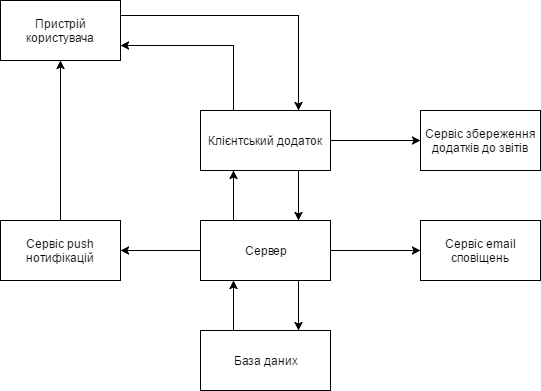
\includegraphics[width=0.75\textwidth]{4_structural_scheme}
	\caption{Структурна схема функціювання системи}
	\label{structural_scheme}
\end{figure}

\subsection{Опис логічної схеми}

Для роботи з багтрекінговою системою обов'язковою умовою є авторизація. Неавторизований користувач в системі має право лише на операції авторизації або реєстрації.

\subsubsection{Авторизація}
Для авторизації користувач повинен здійснити наступні кроки:
\begin{enumerate}
	\item Ввести логін
	\item Ввести пароль
\end{enumerate}

У випадку введення неіснуючого логіну або неправильного паролю користувач буде змушений ввести ці дані заново до тих пір, доки сервер не підтвердить правильніть введених даних.

\begin{figure}[H]
	\centering
	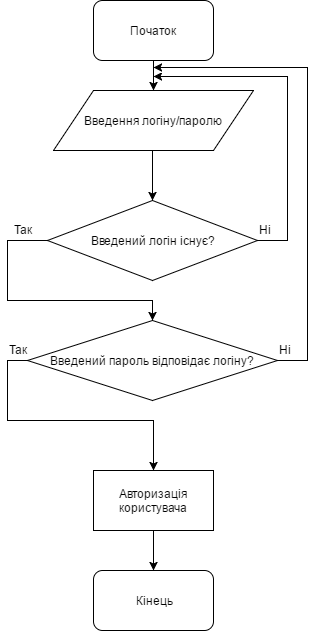
\includegraphics[width=0.4\textwidth]{4_login_flow}
	\caption{Блок-схема авторизації користувача}
\end{figure}

\subsubsection{Реєстрація}
Для реєстрації користувач повинен здійснити наступні кроки:
\begin{enumerate}
	\item Ввести бажаний логін
	\item Ввести бажаний пароль
\end{enumerate}

У випадку вибору зайнятого логіну або занадто слабкого паролю користувач буде змушений ввести ці дані заново до тих пір, доки сервер не підтвердить, що вибраний логін є вільним, а пароль є достатньо сильним.

\begin{figure}[H]
	\centering
	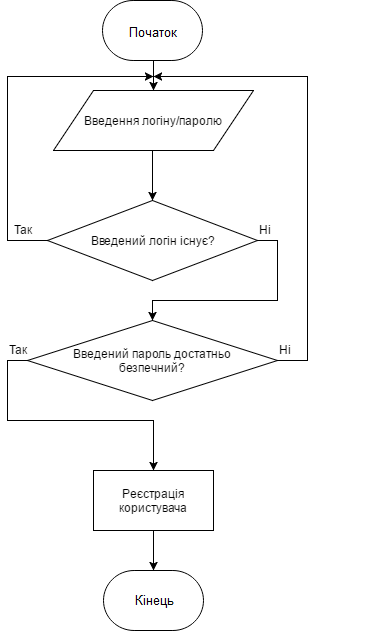
\includegraphics[width=0.4\textwidth]{4_signup_flow}
	\caption{Блок-схема реєстрації користувача}
\end{figure}

\subsubsection{Створення проекту}
Для створення нового проекту користувач повинен здійснити наступні кроки:
\begin{enumerate}
	\item Ввести назву проекту
	\item Ввести которкий опис проекту
	\item (Опціонально) ввести повний опис проекту
\end{enumerate}

У випадку вибору уже існуючої назви проекту або відсутності короткого опису проекту, користувач буде змушений ввести ці дані заново до тих пір, доки сервер не підтвердить, що проекту з такою назвою ще не існує та короткий опис присутній.

\begin{figure}[H]
	\centering
	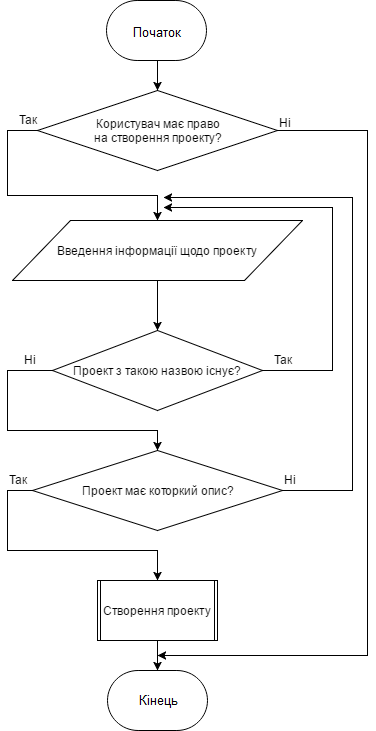
\includegraphics[width=0.75\textwidth]{4_project_creation_flow}
	\caption{Блок-схема створення проекту}
\end{figure}

\subsubsection{Створення звіту}
Для створення нового звіту користувач повинен здійснити наступні кроки:
\begin{enumerate}
	\item Ввести которткий опис проблеми
	\item Обрати тип проблеми
\end{enumerate}

У випадку відсутності короткого опису проблеми або не обраного типу, користувач буде змушений ввести ці дані заново до тих пір, доки сервер не підтвердить, що короткий опис проблеми присутній, а тип обрано.

Також, за бажанням, користувач може виконати одну з таких дій:
\begin{enumerate}
	\item Обрати відповідального за проблему (якщо володіє відповідним правом)
	\item Прикріпити додатки
	\item Ввести повний опис проблеми
	\item Прикріпити додаткову інформацію
\end{enumerate}

\begin{figure}[H]
	\centering
	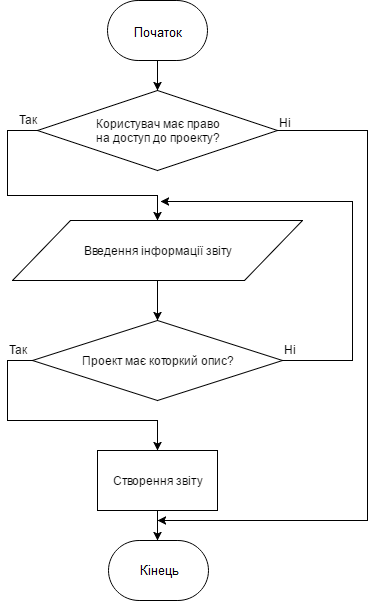
\includegraphics[width=0.75\textwidth]{4_issue_creation_flow}
	\caption{Блок-схема створення звіту}
\end{figure}

\subsection{Розробка бази даних}

База даних системи складається з таких основних сутностей:
\begin{enumerate}
	\item User -- сутність, що уособлює користувача системи.
	\item Project -- сутність, що уособлює проект в системі.
	\item Issue -- сутність, що уособлює звіт в системі.
\end{enumerate}

Серед допоміжних сутностей, що забезпечують роботу системи, є такі:
\begin{enumerate}
	\item Project Member -- сутність, що забезпечує можливість установлення факту участі користувача в проекті.
	\item Permission -- сутність, що забезпечує обмеження можливостей користувачів.
	\item Role -- сутність, що забезпечує можливість групування дозволів на певні дії для забезпечення підтримки рольової структури проектів.
	\item Project Issue -- сутність, що забезпечує можливість нумерації звітів як на рівні всієї системи, так і на рівні окремого проекту.
	\item Issue Type -- сутність, що забезпечує можливість вказування типу звіту.
	\item Issue Status -- сутність, що забезпечує можливість вказувати статус звіту.
	\item Issue Attachment -- сутність, що забезпечує можливість прикріплення додатку до звіту.
\end{enumerate}

\begin{figure}[H]
	\centering
	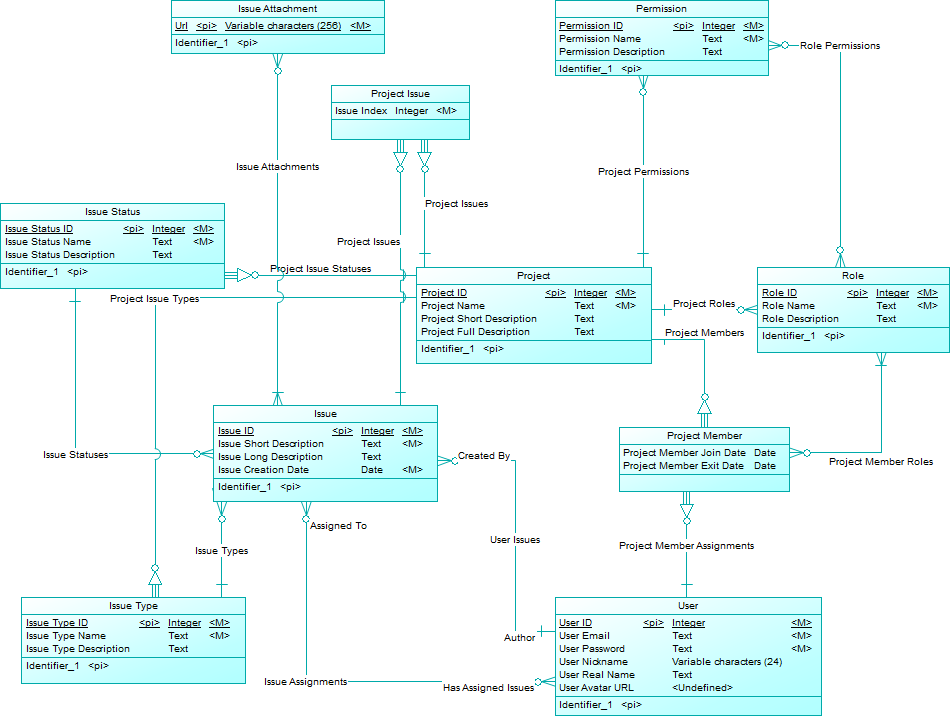
\includegraphics[width=1\textwidth]{4_db_concept}
	\caption{Концептуальна модель бази даних}
\end{figure}

Реалізація багтрекінгової системи потребує пред'являє високі вимоги до побудови бази даних. Для реалізації гнучкої системи, використання зв'язку "багато до багатьох" є необхідною умовою. Концептуальна модель не відображає реальної будови майбутньої бази даних. В реальній базі даних окрім таблиць для вже зазначених вище сутностей будуть ще й такі з'єднувальні таблиці:

\begin{enumerate}
	\item Issue Attachments -- таблиця, що з'єднує звіти з їх додатками.
	\item Role Permissions -- таблиця, що з'єднує ролі з дозволеними діями. Є необхідною складовою реалізації ролей учасників проектів.
	\item Project Member Roles -- таблиця, що з'єднує учасника проекту з присвоєними йому ролями. Є необхідною складовою реалізації ролей учасників проектів.
	\item Issue Assignments -- таблиця, що з'єднує звіт з відповідальним за нього членом команди. Є необхідною складовою реалізації можливості присвоєння декількох відповідальних за звіт осіб.
\end{enumerate}

\begin{figure}[H]
	\centering
	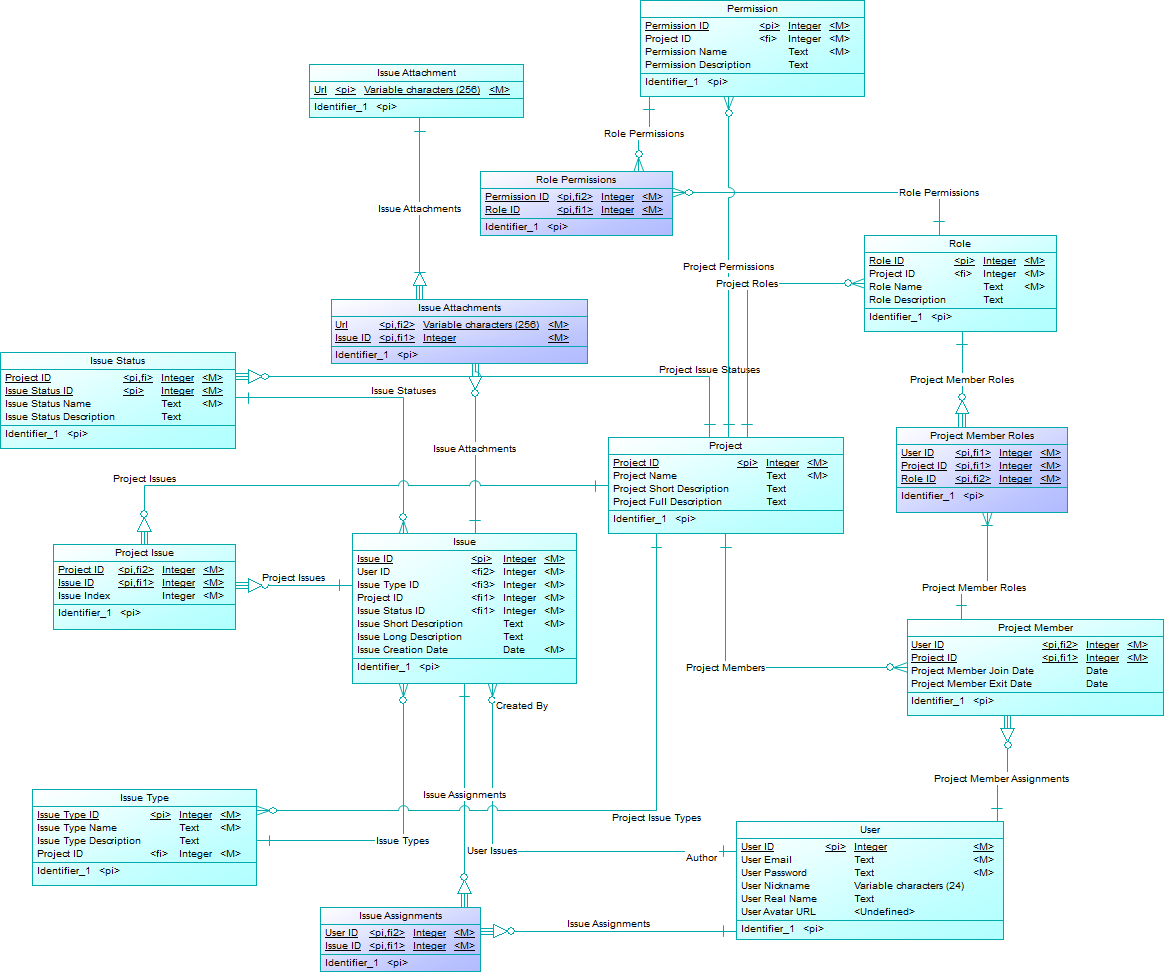
\includegraphics[width=1\textwidth]{4_db_logical}
	\caption{Логічна модель бази даних}
\end{figure}

\begin{figure}[H]
	\centering
	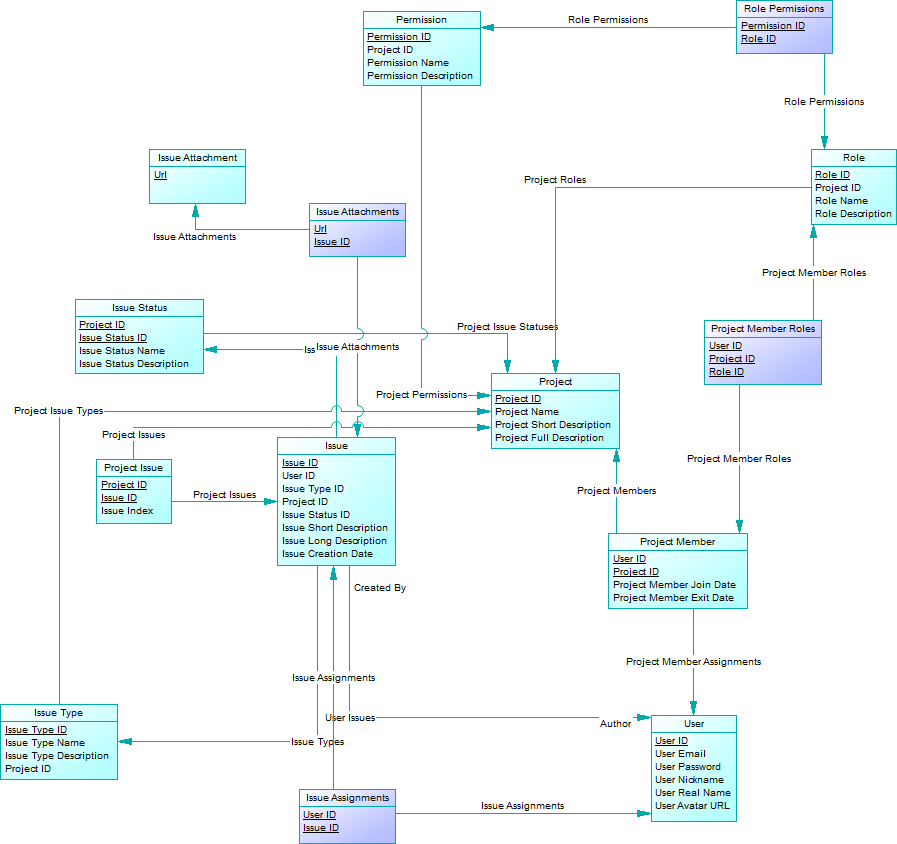
\includegraphics[width=1\textwidth]{4_db_physical}
	\caption{Фізична модель бази даних}
\end{figure}

\subsection{Розробка інтерфейсу користувача}

%TODO: add main app screens screenshots

\subsection{Опис розробки програмних компонентів}

%TODO

\chapter{Тестування інформаційної системи}

%TODO: add tests screenshots

\end{document}